



The number of radians in a 720-degree angle can be written as $a \pi$, where $a$ is a constant. What is the value of $a$ ?

A circle has center $O$, and points $R$ and $S$ lie on the circle. In triangle $O R S$, the measure of $\angle R O S$ is $88^{\circ}$. What is the measure of $\angle R S O$, in degrees? (Disregard the degree symbol when entering your answer.)

In the $x y$-plane, the graph of $2 x^{2}-6 x+2 y^{2}+2 y=45$ is a circle. What is the radius of the circle?\\
A. 5\\
B. 6.5\\
C. $\sqrt{40}$\\
D. $\sqrt{50}$

An angle has a measure of $\frac{9 \pi}{20}$ radians. What is the measure of the angle in degrees?

\section*{ID: a0cacec1}
An angle has a measure of $\frac{16 \pi}{15}$ radians. What is the measure of the angle, in degrees?

\section*{ID: 23c5fcce}
\begin{center}
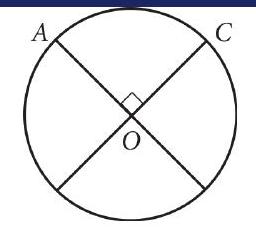
\includegraphics[max width=\textwidth]{2025_06_15_44388a8c3a9d04fd81aag-16}
\end{center}

The circle above with center $O$ has a circumference of 36 . What is the length of minor arc $\wideparen{A C}$ ?\\
A. 9\\
B. 12\\
C. 18\\
D. 36

\section*{ID: f1c1e971}
The measure of angle $R$ is $\frac{2 \pi}{3}$ radians. The measure of angle $T$ is $\frac{5 \pi}{12}$ radians greater than the measure of angle $R$. What is the measure of angle $T$, in degrees?\\
A. 75\\
B. 120\\
C. 195\\
D. 390

\section*{ID: 9acd101f}
The equation $x^{2}+(y-1)^{2}=49$ represents circle A. Circle B is obtained by shifting circle A down 2 units in the $x y$-plane. Which of the following equations represents circle $B$ ?\\
A. msup $+(y-1)^{2}=49$\\
B. $x^{2}+\operatorname{msup}=49$\\
C. $\operatorname{msup}+(y-1)^{2}=49$\\
D. $x^{2}+\operatorname{msup}=49$

\section*{ID: ca2235f6}
A circle has center $O$, and points $A$ and $B$ lie on the circle. The measure of $\operatorname{arc} A B$ is $45^{\circ}$ and the length of arc $A B$ is 3 inches. What is the circumference, in inches, of the circle?\\
A. 3\\
B. 6\\
C. 9\\
D. 24

In the $x y$-plane, a circle with radius 5 has center $(-8,6)$. Which of the following is an equation of the circle?\\
A. $(x-8)^{2}+(y+6)^{2}=25$\\
B. $(x+8)^{2}+(y-6)^{2}=25$\\
c. $(x-8)^{2}+(y+6)^{2}=5$\\
D. $(x+8)^{2}+(y-6)^{2}=5$

Which of the following equations represents a circle in the $x y$-plane that intersects the $y$-axis at exactly one point?\\
A. $\operatorname{msup}+(y-8)^{2}=16$\\
B. msup $+(y-4)^{2}=16$\\
C. msup $+(y-9)^{2}=16$\\
D. $x^{2}+\operatorname{msup}=16$

$$
(x-6)^{2}+(y+5)^{2}=16
$$

In the $x y$-plane, the graph of the equation above is a circle. Point $P$ is on the circle and has coordinates $(10,-5)$. If $\overline{P Q}$ is a diameter of the circle, what are the coordinates of point $Q$ ?\\
A. $(2,-5)$\\
B. $(6,-1)$\\
c. $(6,-5)$\\
D. $(6,-9)$

A circle in the $x y$-plane has its center at $(-5,2)$ and has a radius of 9 . An equation of this circle is $x^{2}+y^{2}+a x+b y+c=0$, where $a, b$, and $c$ are constants. What is the value of $c$ ?

The equation $x^{2}+(y-2)^{2}=36$ represents circle A. Circle B is obtained by shifting circle A down 4 units in the $x y$-plane. Which of the following equations represents circle $B$ ?\\
A. $x^{2}+\operatorname{msup}=36$\\
B. $x^{2}+\operatorname{msup}=36$\\
C. $\operatorname{msup}+(y-2)^{2}=36$\\
D. msup $+(y-2)^{2}=36$

\section*{ID: 95ba2d09}
\begin{center}
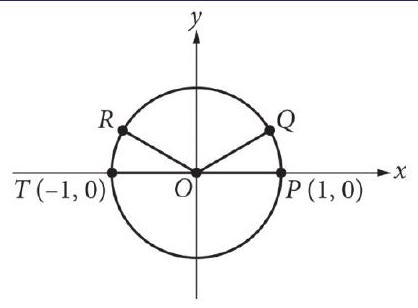
\includegraphics[max width=\textwidth]{2025_06_15_44388a8c3a9d04fd81aag-25}
\end{center}

In the $x y$-plane above, points $P, Q, R$, and $T$ lie on the circle with center $O$. The degree measures of angles $P O Q$ and $R O T$ are each $30^{\circ}$. What is the radian measure of angle QOR ?\\
A. $\frac{5}{6} \pi$\\
B. $\frac{3}{4} \pi$\\
c. $\frac{2}{3} \pi$\\
D. $\frac{1}{3} \pi$\\
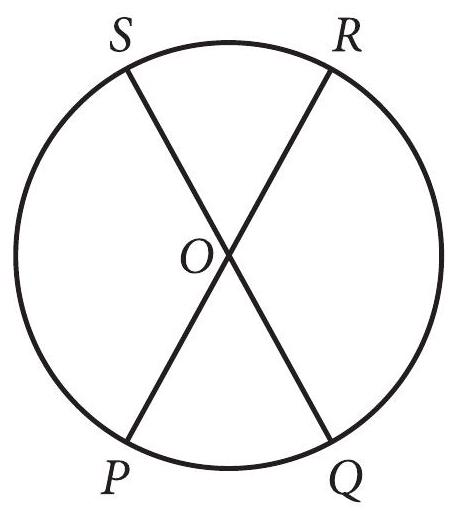
\includegraphics[max width=\textwidth, center]{2025_06_15_44388a8c3a9d04fd81aag-26}

Note: Figure not drawn to scale.\\
The circle shown has center $O$, circumference $144 \pi$, and diameters $\overline{P R}$ and $\overline{Q S}$. The length of arc $P S$ is twice the length of arc $P Q$. What is the length of $\operatorname{arc} Q R$ ?\\
A. $24 \pi$\\
B. $48 \pi$\\
C. $72 \pi$\\
D. $96 \pi$

Points $A$ and $B$ lie on a circle with radius 1 , and $\operatorname{arc} \wideparen{A B}$ has length $\frac{\pi}{3}$. What fraction of the circumference of the circle is the length of arc $\wideparen{A B}$ ?

\section*{ID: acd30391}
A circle in the $x y$-plane has equation $(x+3)^{2}+(y-1)^{2}=25$. Which of the following points does NOT lie in the interior of the circle?\\
A. $(-7,3)$\\
B. $(-3,1)$\\
C. $(0,0)$\\
D. $(3,2)$

A circle in the $x y$-plane has its center at $(-4,5)$ and the point $(-8,8)$ lies on the circle. Which equation represents this circle?\\
A. $\operatorname{msup}+(y+5)^{2}=5$\\
B. $\operatorname{msup}+(y-5)^{2}=5$\\
C. $\operatorname{msup}+(y+5)^{2}=25$\\
D. $\operatorname{msup}+(y-5)^{2}=25$


